\input{preamble-slides169}

%Tick mark commands
\newcommand\ticks{}
  \def\ticks{{Bar[scale=2]}-{Bar[scale=2]}}
\newcommand\paraticks{}
  \def\paraticks{{Straight Barb[reversed, scale=2]}-{Straight Barb[scale=2]}}

\title{Geometry Unit 7: Congruence transformations}
\date{17 January 2023 - 3 February 2023}

\begin{document}
\frame{\titlepage}
\section[Outline]{}
\frame{\tableofcontents}

\section{7.1 Translation \hfill 17 January \,}
\begin{frame}{Learning Target: I can slide a figure}
  {HSG.CO.A.5 Congruence transformations \hfill \alert{7.1 Tuesday 17 January}}
  \begin{columns}
    \column{0.6\textwidth}
    Do Now
    \begin{enumerate}
      \item Review your Jumprope grades
      \item Find the rise and run of the line segment $\overline{AB}$.
    \end{enumerate}
    Lesson: Translation, classwork practice \\
    Homework: Complete the classwork practice
    \column{0.4\textwidth}
    \begin{flushright}
      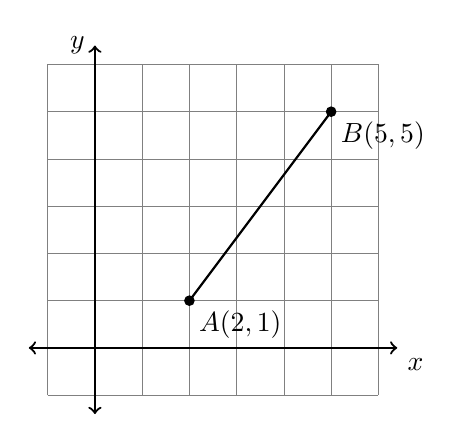
\begin{tikzpicture}[scale=0.6]
        \draw[help lines] (-1,-1) grid (6,6);
        \draw[thick, <->] (-1.4,0) -- (6.4,0) node [below right] {$x$};
        \draw[thick, <->] (0,-1.4)--(0,6.4) node [left] {$y$};
        \draw[thick,domain=2:5] plot (\x, 1.333*\x-1.667);
        \draw [fill] (2,1) circle [radius=0.1] node[below right] {$A(2,1)$};
        \draw [fill] (5,5) circle [radius=0.1] node[below right] {$B(5,5)$};
      \end{tikzpicture}
    \end{flushright}
  \end{columns}
\end{frame}

\begin{frame}{Translation}
    \begin{columns}
      \column{0.6\textwidth}
      Rise is plus 4, run is plus 3. \\
      $$A(2,1) \rightarrow B(5,5)$$
      \begin{description}
        \item[Translate] Move a figure horizontally and vertically (slide)
        \item[Vector] A quantity with both magnitude and direction 
        $$\overrightarrow{AB}=(3,4)$$
      \end{description}
      \column{0.4\textwidth}
      \begin{flushright}
        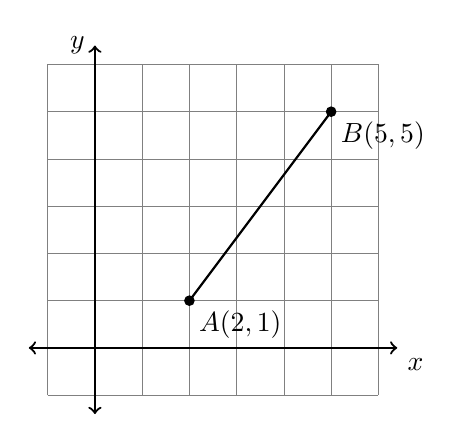
\begin{tikzpicture}[scale=0.6]
          \draw[help lines] (-1,-1) grid (6,6);
          \draw[thick, <->] (-1.4,0) -- (6.4,0) node [below right] {$x$};
          \draw[thick, <->] (0,-1.4)--(0,6.4) node [left] {$y$};
          \draw[thick,domain=2:5] plot (\x, 1.333*\x-1.667);
          \draw [fill] (2,1) circle [radius=0.1] node[below right] {$A(2,1)$};
          \draw [fill] (5,5) circle [radius=0.1] node[below right] {$B(5,5)$};
        \end{tikzpicture}
      \end{flushright}
    \end{columns}
  \end{frame}

\begin{frame}{Example: Translate point $A$ up two units and right four units}
    \begin{columns}
    \column{0.6\textwidth}
        Notation for translation: \\
        $$\overrightarrow{AA'}=(+4,+2)$$
        $$A(1,2) \rightarrow A'(1+4,2+2)$$
        $$T_{+4,+2}$$
        \begin{description}
            \item[Pre-image] The original figure
            \item[Image] The result of a transformation
            \item[$\rightarrow$] We say the $A$ is \emph{mapped} to $A'$.
            \item[Prime] The prime symbol is used to denote the image ($A'$)
          \end{description}
    \column{0.4\textwidth}
    \begin{flushright}
    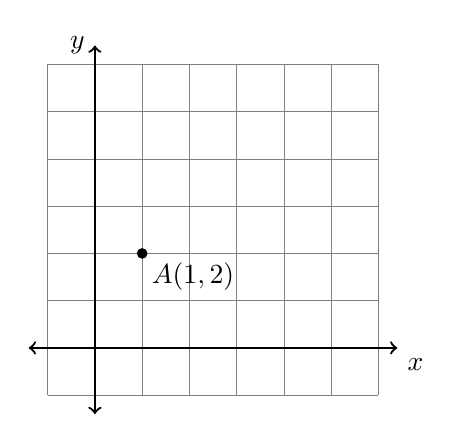
\begin{tikzpicture}[scale=0.6]
        \draw[help lines] (-1,-1) grid (6,6);
        \draw[thick, <->] (-1.4,0) -- (6.4,0) node [below right] {$x$};
        \draw[thick, <->] (0,-1.4)--(0,6.4) node [left] {$y$};
        \draw [fill] (1,2) circle [radius=0.1] node[below right] {$A(1,2)$};
    \end{tikzpicture}
    \end{flushright}
\end{columns}
\end{frame}

\begin{frame}{Translate $\triangle ABC$ right one unit and up three units $T_{+1,+3}$}
    \begin{columns}
    \column{0.6\textwidth}
        $$(x,y) \rightarrow (x+1,y+3)$$
        $$A(1,1) \rightarrow$$
        $$B(1,2) \rightarrow$$
        $$C(4,1) \rightarrow$$

        \begin{description}
            \item[Rigid motion] Move without changing the shape or size (isometry)
            \item[Congruent] Figures with the same size and shape
            \item[Invariant] Does not change (lengths, angles, area, perimeter)
          \end{description}
    \column{0.4\textwidth}
    \begin{flushright}
    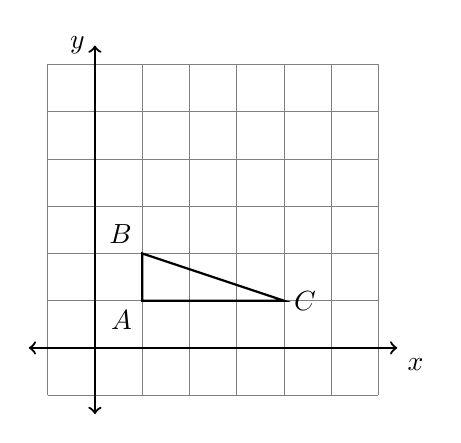
\begin{tikzpicture}[scale=0.6]
        \draw[help lines] (-1,-1) grid (6,6);
        \draw[thick, <->] (-1.4,0) -- (6.4,0) node [below right] {$x$};
        \draw[thick, <->] (0,-1.4)--(0,6.4) node [left] {$y$};
        \draw[thick] (1,2)node[above left]{$B$} --(1,1)node[below left]{$A$} --
            (4,1) node [right] {$C$} --cycle;
    \end{tikzpicture}
    \end{flushright}
\end{columns}
\end{frame}

\section{7.2 Reflection \hfill 18 January \,}
\begin{frame}{Learning Target: I can reflect a figure}
  {HSG.CO.A.5 Congruence transformations \hfill \alert{7.2 Wednesday 18 January}}
  \begin{columns}
    \column{0.6\textwidth}
    Do Now: Find the lengths of the sides of $\triangle ABC$. \\
    $AC=$ \\
    $BC=$ \\
    $AB=$ \\[0.5cm]
    Lesson: Reflection, classwork practice \\
    Homework: Complete classwork, Deltamath assignment
    \column{0.4\textwidth}
    \begin{flushright}
      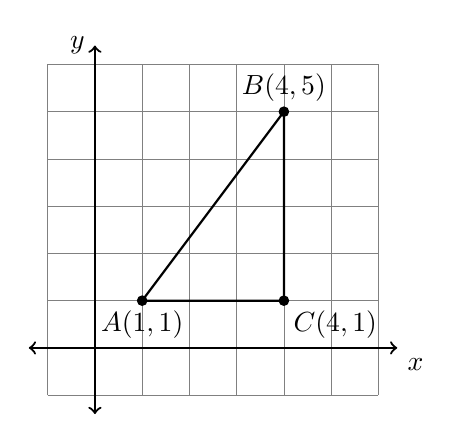
\begin{tikzpicture}[scale=0.6]
        \draw[help lines] (-1,-1) grid (6,6);
        \draw[thick, <->] (-1.4,0) -- (6.4,0) node [below right] {$x$};
        \draw[thick, <->] (0,-1.4)--(0,6.4) node [left] {$y$};
        \draw[thick] (1,1)--(4,5)--(4,1)--cycle;
        \draw [fill] (1,1) circle [radius=0.1] node[below] {$A(1,1)$};
        \draw [fill] (4,5) circle [radius=0.1] node[above] {$B(4,5)$};
        \draw [fill] (4,1) circle [radius=0.1] node[below right] {$C(4,1)$};
      \end{tikzpicture}
    \end{flushright}
  \end{columns}
\end{frame}

\begin{frame}{Reflect or flip an object across the $y$-axis}
  {Reflection is a rigid motion.}
  \begin{columns}
    \column{0.5\textwidth}
    $$\triangle ABC \rightarrow \triangle A'B'C'$$
      \begin{description}
        \item[Reflection] A transformation that flips an object across a line
        \item[Line of reflection] The line across which the object is flipped
        \item[Correspond] Parts that map to each other \\
        $A$ corresponds to $A'$.
      \end{description}
      
    \column{0.5\textwidth}
    \begin{flushright}
      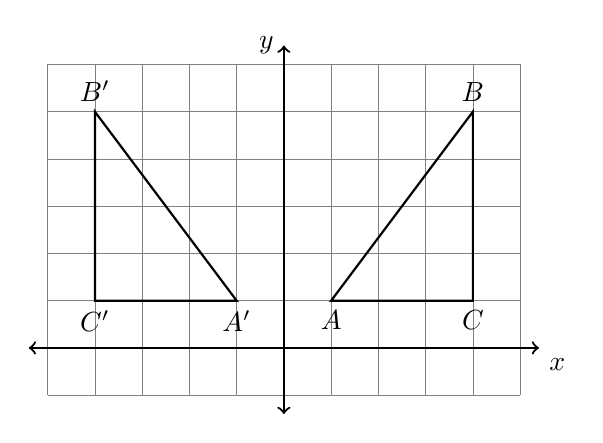
\begin{tikzpicture}[scale=0.6]
        \draw[help lines] (-5,-1) grid (5,6);
        \draw[thick, <->] (-5.4,0) -- (5.4,0) node [below right] {$x$};
        \draw[thick, <->] (0,-1.4)--(0,6.4) node [left] {$y$};
        \draw[thick] (1,1)node[below] {$A$}--
          (4,5)node[above] {$B$}--
          (4,1)node[below] {$C$}--cycle;
        \draw[thick] (-1,1)node[below] {$A'$}--
          (-4,5)node[above] {$B'$}--
          (-4,1)node[below] {$C'$}--cycle;
      \end{tikzpicture}
    \end{flushright}
  \end{columns}
\end{frame}

\section{7.3 Rotation \hfill 20 January \,}
\begin{frame}{Learning Target: I can rotate a figure}
  {HSG.CO.A.5 Congruence transformations \hfill \alert{7.3 Friday 20 January}}
  \begin{columns}
    \column{0.6\textwidth}
    Do Now: Find the angle measures of right $\triangle ABC$. \\
    m$\angle A= 30^\circ$ \\
    m$\angle B=$ \\
    m$\angle C=$ \\[0.5cm]
    Lesson: Rotation, classwork practice \\
    Homework: Complete classwork, Deltamath assignment
    \column{0.4\textwidth}
    \begin{flushright}
      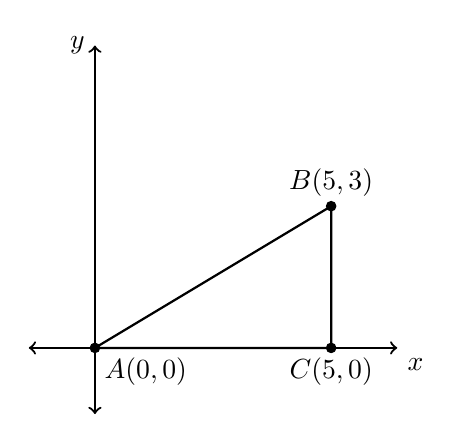
\begin{tikzpicture}[scale=0.6]
        \draw[thick, <->] (-1.4,0) -- (6.4,0) node [below right] {$x$};
        \draw[thick, <->] (0,-1.4)--(0,6.4) node [left] {$y$};
        \draw[thick] (0,0)--(5,3)--(5,0)--cycle;
        \draw [fill] (0,0) circle [radius=0.1] node[below right] {$A(0,0)$};
        \draw [fill] (5,3) circle [radius=0.1] node[above] {$B(5,3)$};
        \draw [fill] (5,0) circle [radius=0.1] node[below] {$C(5,0)$};
      \end{tikzpicture}
    \end{flushright}
  \end{columns}
\end{frame}

\section{7.4 Rotation \hfill 23 January \,}
\begin{frame}{Learning Target: I can employ multiple rigid motions}
  {HSG.CO.A.5 Congruence transformations \hfill \alert{7.4 Friday 20 January}}
  Do Now: Rotate $\triangle ABC$ counterclockwise $90^\circ$ around the origin.  \vspace{0.5cm}
  \begin{columns}
    \column{0.5\textwidth}
    $A(0,0) \rightarrow$ \\[0.3cm]
    $B(4,3) \rightarrow$ \\[0.3cm]
    $C(4,0) \rightarrow$ \\[0.3cm]
    Lesson: Composition of transformations, mixed practice \\[0.5cm]
    Homework: Complete classwork, Deltamath assignment
    \column{0.5\textwidth}
    \begin{flushright}
      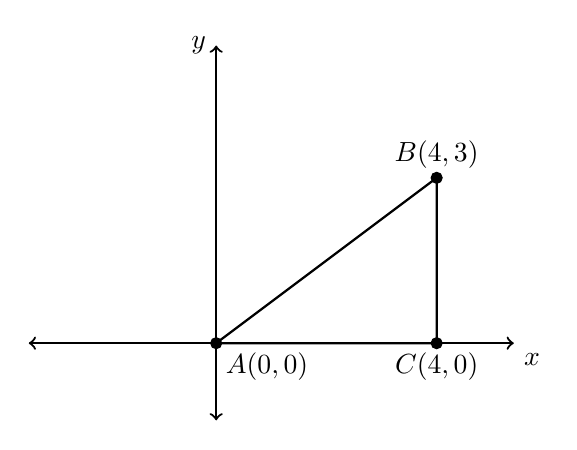
\begin{tikzpicture}[scale=0.7]
        \draw[thick, <->] (-3.4,0) -- (5.4,0) node [below right] {$x$};
        \draw[thick, <->] (0,-1.4)--(0,5.4) node [left] {$y$};
        \draw[thick] (0,0)--(4,3)--(4,0)--cycle;
        \draw [fill] (0,0) circle [radius=0.1] node[below right] {$A(0,0)$};
        \draw [fill] (4,3) circle [radius=0.1] node[above] {$B(4,3)$};
        \draw [fill] (4,0) circle [radius=0.1] node[below] {$C(4,0)$};
      \end{tikzpicture}
    \end{flushright}
  \end{columns}
\end{frame}

\begin{frame}{Learning Target: I can employ multiple rigid motions}
  Solution: Rotate $\triangle ABC$ counterclockwise $90^\circ$ around the origin.  \vspace{0.5cm}
  \begin{columns}
    \column{0.5\textwidth}
      $A(0,0) \rightarrow A'(0,0)$ \\[0.3cm]
      $B(4,3) \rightarrow B'(-3,4)$ \\[0.3cm]
      $C(4,0) \rightarrow C'(0,4)$ \\[0.3cm]
    \column{0.5\textwidth}
    \begin{flushright}
      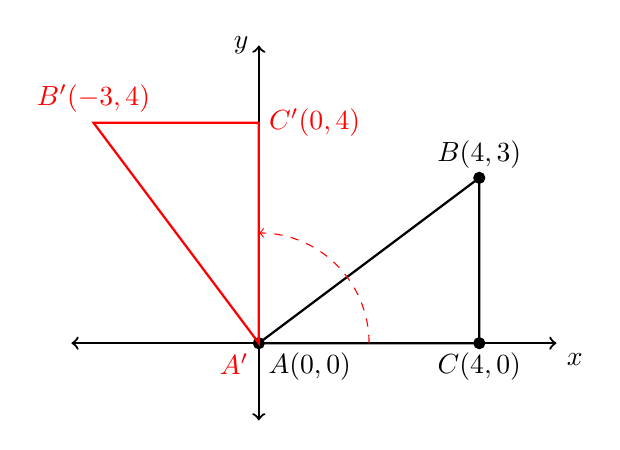
\begin{tikzpicture}[scale=0.7]
        \draw[thick, <->] (-3.4,0) -- (5.4,0) node [below right] {$x$};
        \draw[thick, <->] (0,-1.4)--(0,5.4) node [left] {$y$};
        \draw[thick] (0,0)--(4,3)--(4,0)--cycle;
        \draw [fill] (0,0) circle [radius=0.1] node[below right] {$A(0,0)$};
        \draw [fill] (4,3) circle [radius=0.1] node[above] {$B(4,3)$};
        \draw [fill] (4,0) circle [radius=0.1] node[below] {$C(4,0)$};
        \draw[thick, red] (0,0)node[below left]{$A'$}--
          (-3,4)node[above]{$B'(-3,4)$}--
          (0,4)node[right]{$C'(0,4)$}--cycle;
        \draw[dashed,->,red] (2,0) arc (0:90:2);
      \end{tikzpicture}
    \end{flushright}
  \end{columns}
\end{frame}

\begin{frame}{A \emph{composition} is multiple transformations, one after the other}
  Example: Translate $\triangle ABC$ to the right 5 units then reflect it over the $x$-axis.
  \begin{columns}
    \column{0.5\textwidth}
    $ \hspace{1cm} T_{+5,0} \hspace{1cm} reflect_{ x-axis}$ \\[0.3cm]
    $A(-1,2) \rightarrow A'(4,2) \rightarrow A'(4,-2)$ \\[0.3cm]
    $B(-4,3) \rightarrow B'(1,3) \rightarrow B'(1,-3)$ \\[0.3cm]
    $C(-4,2) \rightarrow C'(1,2) \rightarrow C'(1,-2)$ \\[0.3cm]
    \column{0.5\textwidth}
    \begin{flushright}
      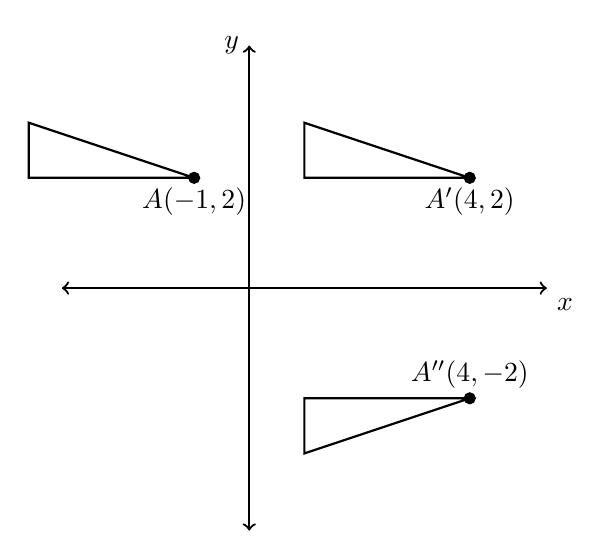
\begin{tikzpicture}[scale=0.7]
        \draw[thick, <->] (-3.4,0) -- (5.4,0) node [below right] {$x$};
        \draw[thick, <->] (0,-4.4)--(0,4.4) node [left] {$y$};
        \draw[thick] (-1,2)--(-4,2)--(-4,3)--cycle;
        \draw [fill] (-1,2) circle [radius=0.1] node[below] {$A(-1,2)$};
        \draw [fill] (4,2) circle [radius=0.1] node[below] {$A'(4,2)$};
        \draw [fill] (4,-2) circle [radius=0.1] node[above] {$A''(4,-2)$};
        \draw[thick] (4,2)--(1,2)--(1,3)--cycle;
        \draw[thick] (4,-2)--(1,-2)--(1,-3)--cycle;
      \end{tikzpicture}
    \end{flushright}
  \end{columns}
\end{frame}

\end{document}